\documentclass{beamer} %[12pt]
\usepackage{xcolor}
%\usetheme{boadilla}
%\usetheme{malmoe}
%\usetheme{copenhagen}
%\usecolortheme{rose}
\usecolortheme{beaver}
\usepackage{pgf, graphics}
\usepackage{graphicx}
%\usepackage[left=3cm,top=3cm,right=3cm,nohead,nofoot]{geometry}
\usepackage{hyperref}
\usepackage{setspace}
\usepackage[square]{natbib}
\usepackage{amsmath}
\usepackage{amssymb}
\usepackage{verbatim}
\usepackage{color}
\usepackage{fancyvrb}
\usepackage{bbm}

\begin{filecontents}{ref.bib}
\end{filecontents}

%\usetheme{EastLansing}
%\usepackage{natbib}
\bibliographystyle{apalike}
% make bibliography entries smaller
%\renewcommand\bibfont{\scriptsize}
% If you have more than one page of references, you want to tell beamer
% to put the continuation section label from the second slide onwards
\setbeamertemplate{frametitle continuation}[from second]
% Now get rid of all the colours
\setbeamercolor*{bibliography entry title}{fg=black}
\setbeamercolor*{bibliography entry author}{fg=black}
\setbeamercolor*{bibliography entry location}{fg=black}
\setbeamercolor*{bibliography entry note}{fg=black}
% and kill the abominable icon
\setbeamertemplate{bibliography item}{}


\newcommand{\hl}[1]{\colorbox{yellow}{#1}}
\newcommand{\hlblue}[1]{\colorbox{green}{#1}}
\newcommand{\hlblu}[1]{\colorbox{cyan}{#1}}
\newcommand{\hlred}[1]{\colorbox{cyan}{#1}}
\newcommand{\hlre}[1]{\colorbox{pink}{#1}}
\newcommand{\hlgreen}[1]{\colorbox{pink}{#1}}
\newcommand{\hlgree}[1]{\colorbox{green}{#1}}



\DeclareMathOperator*{\argmax}{\arg\!\max}

\DeclareMathOperator*{\argmin}{\arg\!\min}


\newcommand{\specialcell}[2][c]{%
  \begin{tabular}[#1]{@{}c@{}}#2\end{tabular}}



%\setbeamersize{text margin left=.5cm,text margin right=.5cm}
\newenvironment{changemargin}[2]{%
  \begin{list}{}{%
    \setlength{\topsep}{0pt}%
    \setlength{\leftmargin}{#1}%
    \setlength{\rightmargin}{#2}%
    \setlength{\listparindent}{\parindent}%
    \setlength{\itemindent}{\parindent}%
    \setlength{\parsep}{\parskip}%
  }%
  \item[]}{\end{list}}
\setbeamertemplate{navigation symbols}{}%remove navigation symbols
\usepackage{color}
\newcommand{\hilight}[1]{\colorbox{yellow}{#1}}
\setbeamertemplate{footline}[page number]

\begin{document}


\title[dedup]{Today:  What Is Data?\\Graphics Principles\\Friday:  Introduction to R and Reproducibility\\Monday:  No class (Labor Day)}


\author[Samuel L. Ventura]{\\
  \large{Sam Ventura\\36-315}}
\institute[CMU Statistics]{Department of Statistics\\Carnegie Mellon University}
\date{\today}


\begin{frame}
	\maketitle
	
\end{frame}



\begin{frame}\frametitle{What Is Data?}
	\centering
	
\end{frame}


\begin{frame}\frametitle{How Do We Describe Data?}
	Two measurements used to describe datasets:
	
	\vskip 3 cm
	
	Data is usually in matrix form:
	
	\vskip 3 cm
	
\end{frame}


\begin{frame}\frametitle{Types of Data}
	
	Categorical:
	
	\vskip 4 cm
	
	Continuous:
	
	\vskip 4 cm
	
\end{frame}


\begin{frame}\frametitle{Graphics and Their Goals (from Tufte)}
	\small
	
	Graphics:  visually display measured quantities by combining points, lines, coordinate system, numbers, symbols, words, shading, color
	
	\vskip 0.25 cm
	
	Goals:  show data!
	
	\begin{itemize}
		\item induce viewer to think about substance, not graphical methodology
		\item avoid \textbf{distorting} the data
		\item present numbers in small space
		\item make large, complicated datasets more coherent
		\item encourage comparison of different pieces of data
		\item reveal data at several levels of detail
		\item describe, explore, tabulate, or decorate
		\item be closely integrated with statistical/verbal descriptions of dataset
	\end{itemize}
	
	Graphs that do not meet these goals are not successful
	
	\vskip 0.25 cm
	
	Graphs leading viewers to make misleading conclusions should be avoided
	
\end{frame}



\begin{frame}\frametitle{Distortion = ``graph doesn't match the data''}
	\small
	
	Visual representation of data is inconsistent with numerical representation
	
	\vskip 0.10 cm

	\vskip 0.10 cm
	
	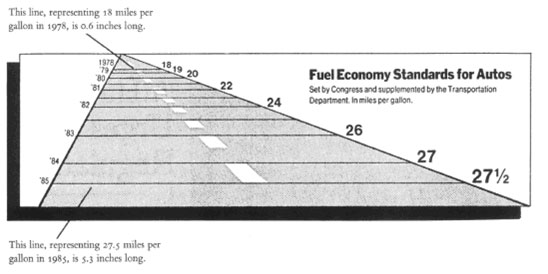
\includegraphics[width=0.71\linewidth]{fuel.jpg}
	
	Tufte suggests optimizing the Lie Factor:
	
	\vskip 10 cm
	
\end{frame}




\begin{frame}\frametitle{``Decorating'' and Data-Ink}
	\small
	
	Graphics should not draw the viewer's attention away from the data.  Extras get in the way.
	
	\vskip 0.25 cm
	
	\textbf{Note:  Decoration does not refer to appropriate graph labeling.}  Labels should always be clear, detailed, and thorough.  \\Label key parts of the data.  Add text explanations if necessary.
	
	\vskip 0.25 cm
	
	\textbf{Data Ink should primarily present information about the data:}  \\the non-erasable, non-redundant core of a graphic
	
	\vskip 0.25 cm
	
	Tufte suggests using the \emph{data-ink ratio}:
	
	\vskip 3 cm
\end{frame}



\begin{frame}\frametitle{``Decorating'' / Data-Ink}
	\small
	
	Two ways to increase the proportion of data-ink:
	
	\vskip 0.25 cm
	
	\textbf{Remove non-data-ink:}  
	
	
	\vskip 2 cm
	
	\textbf{Remove redundant data-ink:} \\ 
	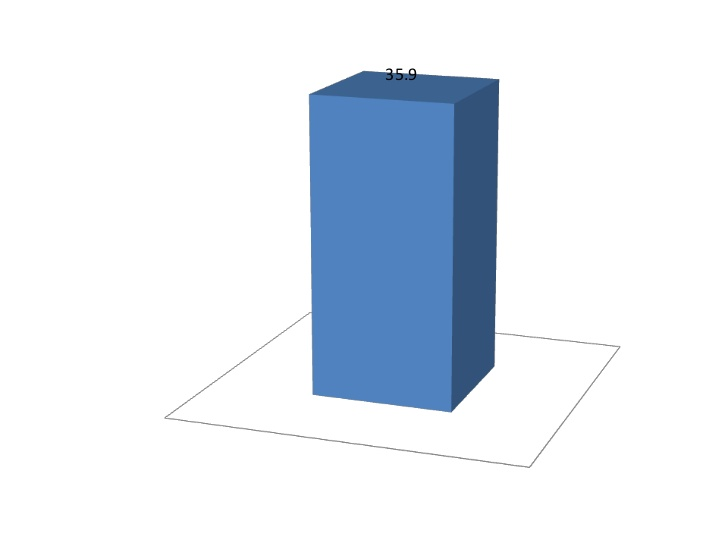
\includegraphics[width = 0.6\linewidth]{data-ink.jpg}
	
	\vskip 3 cm
\end{frame}



\end{document}
